\documentclass[UTF8,a4paper,10pt]{ctexart}
\usepackage[left=2.50cm, right=2.50cm, top=2.50cm, bottom=2.50cm]{geometry} %页边距
\CTEXsetup[format={\Large\bfseries}]{section} %设置章标题居左
 
 
%%%%%%%%%%%%%%%%%%%%%%%
% -- text font --
% compile using Xelatex
%%%%%%%%%%%%%%%%%%%%%%%
% -- 中文字体 --
%\setmainfont{Microsoft YaHei}  % 微软雅黑
%\setmainfont{YouYuan}  % 幼圆    
%\setmainfont{NSimSun}  % 新宋体
%\setmainfont{KaiTi}    % 楷体
%\setmainfont{SimSun}   % 宋体
%\setmainfont{SimHei}   % 黑体
% -- 英文字体 --
%\usepackage{times}
%\usepackage{mathpazo}
%\usepackage{fourier}
%\usepackage{charter}
\usepackage{helvet}
 

\usepackage{amsmath, amsfonts, amssymb} % math equations, symbols
\usepackage[english]{babel}
\usepackage{color}      % color content
\usepackage{graphicx}   % import figures
\usepackage{url}        % hyperlinks
\usepackage{bm}         % bold type for equations
\usepackage{multirow}
\usepackage{booktabs}
\usepackage{epstopdf}
\usepackage{epsfig}
\usepackage{algorithm}
\usepackage{algorithmic}
\renewcommand{\algorithmicrequire}{ \textbf{Input:}}     % use Input in the format of Algorithm  
\renewcommand{\algorithmicensure}{ \textbf{Initialize:}} % use Initialize in the format of Algorithm  
\renewcommand{\algorithmicreturn}{ \textbf{Output:}}     % use Output in the format of Algorithm  
 
 
%\usepackage{fancyhdr} %设置页眉、页脚
%\pagestyle{fancy}
%\lhead{}
%\chead{}
%\rhead{\includegraphics[width=1.2cm]{fig/ZJU_BLUE.eps}}
%\lfoot{}
%\cfoot{}
%\rfoot{}
 


\usepackage{hyperref} %bookmarks
\hypersetup{colorlinks, bookmarks, unicode} %unicode
\usepackage{ctex}
\pagestyle{plain}
\begin{document}
 \renewcommand\figurename{图}
\ctexset{
abstractname = {摘要},
bibname = {参考文献}
}


 
\begin{abstract}
细粒度视觉分类(FGVC)
\end{abstract}
 
 
\section{背景介绍}
人的眼睛是一个很


FGVC在我们的日常

\section{研究现状}


\section{原理和方案}
深度学习在机器视觉领域中广泛应用于细粒度分类任务,下边介绍一下它的原理和方案。


\section{关键技术}
\subsection{模型}
\subsubsection{vision-Transformer}

\subsubsection{MetaFormer}
MetaFormer\cite{diao2022metaformer}这是一个对机器视觉任务非常有用的网络架构,它将视觉信息和元信息结合起来。MetaFormer设计了一个五阶段的网络结构。第一阶段S0是一个简单的三层卷积结构。S1和S2是MBConv块\cite{sandler2018mobilenetv2},具有挤压式激励。MBConv块是基于一个倒置的残差机制和一个瓶颈设计。倒置残差结构的设计是为了提供更高的非线性表示能力,同时保持模型的轻量级,而瓶颈使用较小的中间层来减少计算量。S3和S4是具有相对位置偏置的变换器块。这种偏置缓解了输入序列中的标记顺序不能用于自我注意操作的问题。MetaFormer的工作流程见图\ref{figure 2}。
\begin{figure}[h]
  \centering
  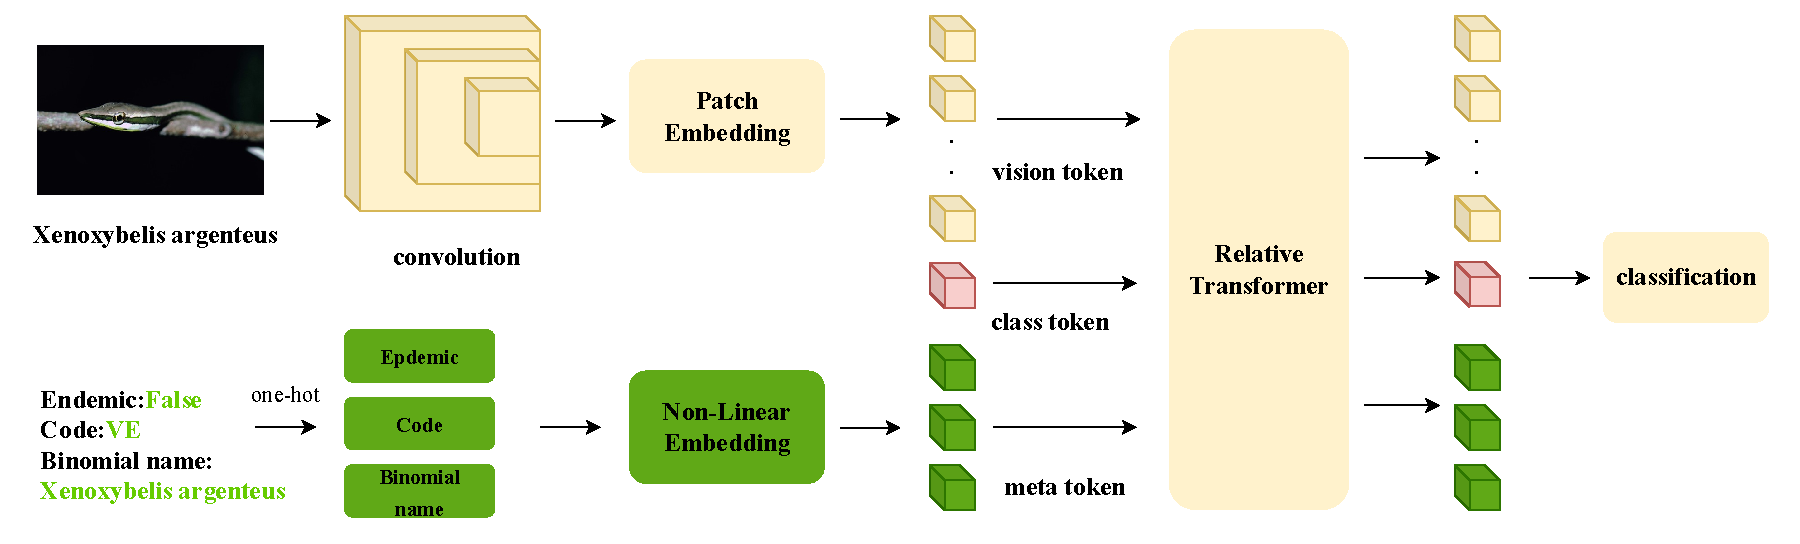
\includegraphics[width=\linewidth]{fig/model.pdf}
  \caption{该模型采用卷积层来提取视觉特征,然后通过Patch Embedding将图像特征转化为视觉标记。Code、Endemic和Binomial name的元信息被热编码,并通过Non-Liner Embedding获得元标记。视觉令牌、元令牌和类令牌使用相对转换层进行融合。融合后的标记在下面的注意区块中被连续聚合。最终输出的类标记用于类别预测。}
\label{figure 2}
\end{figure}



\subsection{损失函数}







 
\bibliographystyle{unsrt}
\bibliography{lunwen}
\end{document} 